% XeLaTeX

\documentclass{article}
\usepackage{ctex}
\usepackage{xypic}
\usepackage{amsfonts,amssymb}
\usepackage{multirow}
\usepackage{geometry}
\usepackage{graphicx}
\usepackage{listings}
\usepackage{lipsum}
\usepackage{courier}
\usepackage{fancyvrb}
\usepackage{etoolbox}


\linespread{1.2}
\geometry{left=3cm,right=2.5cm,top=2.5cm,bottom=2.5cm}

\makeatletter
\patchcmd{\FV@SetupFont}
  {\FV@BaseLineStretch}
  {\fontencoding{T1}\FV@BaseLineStretch}
  {}{}
\makeatother

\lstset{basicstyle=\small\fontencoding{T1}\ttfamily,breaklines=true}
\lstset{numbers=left,frame=shadowbox,tabsize=4}
%\lstset{extendedchars=false}
\begin{document}

\title{实验二 \ 加载用户程序的监控程序 \ 实验报告}
\author {数据科学与计算机学院 \ 计算机科学与技术 2016 级 \\ 王凯祺 \ 16337233}
\maketitle

\section{实验目的}

\begin{itemize}
\item 掌握常用的 BIOS 调用
\item 掌握 BIOS 编程
\item 掌握加载用户程序的方法
\end{itemize}

\section{实验要求}

设计四个有输出的用户可执行程序,分别在屏幕1/4区域动态输出字符,如将用字符 'A' 从屏幕左边某行位置 45 度角下斜射出,保持一个可观察的适当速度直线运动,碰到屏幕相应 $\frac{1}{4}$ 区域的边后产生反射,改变方向运动,如此类推,不断运动;在此基础上,增加你的个性扩展,如同时控制两个运动的轨迹,或炫酷动态变色,个性画面,如此等等,自由不限。还要在屏幕某个区域特别的方式显示你的学号姓名等个人信息。

修改参考原型代码,允许键盘输入,用于指定运行这四个有输出的用户可执行程序之一,要确保系统执行代码不超过512字节,以便放在引导扇区 。

自行组织映像盘的空间存放四个用户可执行程序。

\section{实验过程和结果}

本实验需要使用 NASM 汇编器、WinHex 软件和虚拟机。

\subsection{程序功能}

输入 '1' ,会运行一个在左上角弹球的程序

输入 '2' ,会运行一个在右上角弹球的程序

输入 '3' ,会运行一个在左下角弹球的程序

输入 '4' ,会运行一个在右下角弹球的程序


\subsection{重写 stone.asm }

本次实验要求写 4 个用户程序,分别是在屏幕的 4 个 $\frac{1}{4}$ 区域中弹来弹去。我本想在老师给的 stone.asm 中直接修改,却发现老师只考虑了边反射的情况,没有考虑四个角反射的情况,这会导致字符从角飞出,在屏幕中乱飞。

为了从根本上解决这个问题,我使用了新的方法来写这个程序。

设屏幕为 $n \times m$ 的矩形。我们不妨把 $x$ 坐标和 $y$ 坐标分开来单独考虑。

考虑 $x$ 坐标,每次运动就是 $+1$ 或者 $-1$ ,从 $0$ 开始加到 $n - 1$ ,然后再从 $n - 1$ 减到 $0$ ,周期为 $2n - 2$ 。也就是说, $x$ 坐标每走 $2n - 2$ 步就会回到原点。

设从开始到现在的时间为 $t$ ,那么 $x$ 坐标就是从 $0$ 位置开始走 $t \text{ mod } (2n - 2)$ 步。不难推出 $x$ 的表达式 $x = (t \text{ mod }(2n - 2) < n) ? (t \text{ mod }(2n - 2)) : (2n - 2 - (t \text{ mod }(2n - 2)))$ 。

所以老师的代码可以被大大地简化。少去了分类讨论,减少了出错的可能性。每次只需要将 t 自增 1 ,然后重新计算 $x$ 坐标和 $y$ 坐标即可。

\begin{lstlisting}[language={[x86masm]Assembler}]
	n equ 12

	xor dx, dx                ; clear dx and prepare for division
	mov word ax, [t]          ; ax = t
	xor bx, bx                ; bx register stores divisor
	mov word bx, n
	add bx, bx
	sub bx, 2                 ; bx = 2n - 2
	div bx                    ; dx = t mod (2n - 2)
	cmp dx, n                 ; compare dx and n
	jb xok                    ; if (dx < n) jump xok
	sub bx, dx
	mov dx, bx                ; dx = 2n - 2 - dx
xok:
	mov word [x], dx          ; dx is answer to the x coordinate for time t
\end{lstlisting}

使用这种做法来计算 $x$ 坐标和 $y$ 坐标还有个好处就是,可以非常方便地调整显示区域。例如,我想在屏幕右下角 $\frac{1}{4}$ 显示这个图形,那么只需把 $n$ 改为 12 ,并在上面代码 15 行前加上 add dx, 13 即可。这样,只需要修改几个字符,就可以将显示区域调整到屏幕的任何位置了。

\subsection{编写 myos.asm }

除了 4 个用户程序以外,还需要有引导扇区的 bootloader 。我们需要使用 int 13h 读取扇区,并把它放到内存合适的位置上。

\begin{lstlisting}[language={[x86masm]Assembler}]
org  7c00h		; BIOS将把引导扇区加载到0:7C00h处,并开始执行
OffSetOfUserPrg1 equ 0a100h
Start:
	mov	ax, cs	       ; 置其他段寄存器值与CS相同
	mov	ds, ax	       ; 数据段
	mov	bp, Message	   ; BP=当前串的偏移地址
	mov	ax, ds		   ; ES:BP = 串地址
	mov	es, ax		   ; 置ES=DS
	mov	cx, MessageLength  ; CX = 串长
	mov	ax, 1301h		 ; AH = 13h(功能号)、AL = 01h(光标置于串尾)
	mov	bx, 0007h		 ; 页号为0(BH = 0) 黑底白字(BL = 07h)
    mov dh, 0		       ; 行号=0
	mov	dl, 0			 ; 列号=0
	int	10h			 ; BIOS的10h功能:显示一行字符
read:
	mov ah, 0
	int 16h          ; 读取字符
	cmp al, '1'
	jl read
	cmp al, '4'
	jg read
	mov ah, 0        ; 若字符在 '1' 到 '4' 之间,开始执行相应的用户程序
	sub ax, '1'
	mov byte [x], al
	
LoadnEx:
	;读软盘或硬盘上的若干物理扇区到内存的ES:BX处:
	mov ax,cs                ;段地址 ; 存放数据的内存基地址
	mov es,ax                ;设置段地址(不能直接mov es,段地址)
	mov bx, OffSetOfUserPrg1  ;偏移地址; 存放数据的内存偏移地址
	mov cx, bx
	mov ah,2                 ; 功能号
	mov al,1                 ;扇区数
	mov dl,0                 ;驱动器号 ; 软盘为0,硬盘和U盘为80H
	mov dh,0                 ;磁头号 ; 起始编号为0
	mov ch,0                 ;柱面号 ; 起始编号为0
	mov byte cl,[x]          ;根据用户输入,决定扇区号
	add cl,2                 ;起始扇区号 ; 起始编号为1
	int 13H ;                调用读磁盘BIOS的13h功能
	; 用户程序a.com已加载到指定内存区域中
	jmp OffSetOfUserPrg1
AfterRun:
	jmp Start                      ;无限循环
	x db 0
	Message db 'Welcome to MyOS!'
	MessageLength equ ($-Message)
	times 510-($-$$) db 0
	db 0x55,0xaa
\end{lstlisting}


\newpage

\subsection{运行结果}

\begin{figure}[!hbp]
	\centering
	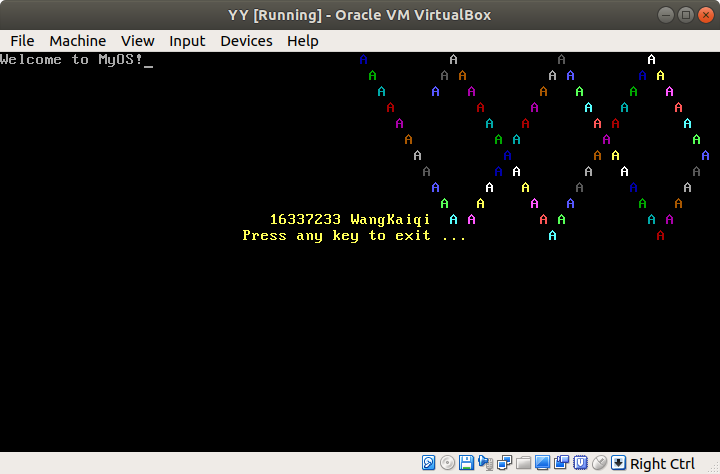
\includegraphics[scale=0.6]{pics/1.png}
\end{figure}


\section{实验总结}

这次实验我只能说是基本完成了吧,因为没有达到我的目的。我希望我的操作系统能够真正地控制用户程序。操作系统能调用程序,程序也能通过中断返回操作系统。我一直没有找到调用程序及程序返回的方法。由于调用程序是直接使用 jmp 指令,程序返回时如果使用中断的 int 21h 将控制权交给控制台,机器就会死机。这是因为 jmp 指令并没有创建一个进程,而只是单纯地把 PC 定向到对应地址,期间并没有保存返回地址等信息。

我尝试了去各个搜索引擎搜索有关“程序返回”“PSP”的资料,很遗憾没有找到标准的调用程序和程序返回的方法。在本实验,我只能创造一种比较偷懒的做法:

1. 使用 jmp 直接跳转到用户程序入口。这种做法的优点是:简单方便,只需一条指令。但这种方法会使操作系统丢失它的控制权。跳转指令执行后,所有控制权都到用户手上了。除非用户转移回操作系统,操作系统永远都不能再获得控制权。

2. 修改用户程序,并在用户程序的最后加上 jmp 7c00 无条件转移到操作系统入口来实现返回。而对于操作系统来说,使用这种方法来返回是非常致命的,因为这样会带来很多安全问题,比如用户的程序能随便转移到操作系统的内核代码。不仅如此,这种方法还增加了管理成本。用户在设计程序时,还要与操作系统设计者商量将程序挂载到哪里去,去修改 org 那行伪指令。

\end{document}
















